
\chapter{Applications: the costs of taxation}

\section{The deadweight loss of taxation}

Figure \ref{fig:the-effect-of-a-tax} show the effect of a tax.
A tax on a good causes the size of the market for the good to shrink.

\begin{figure}[!ht]
  \centering
  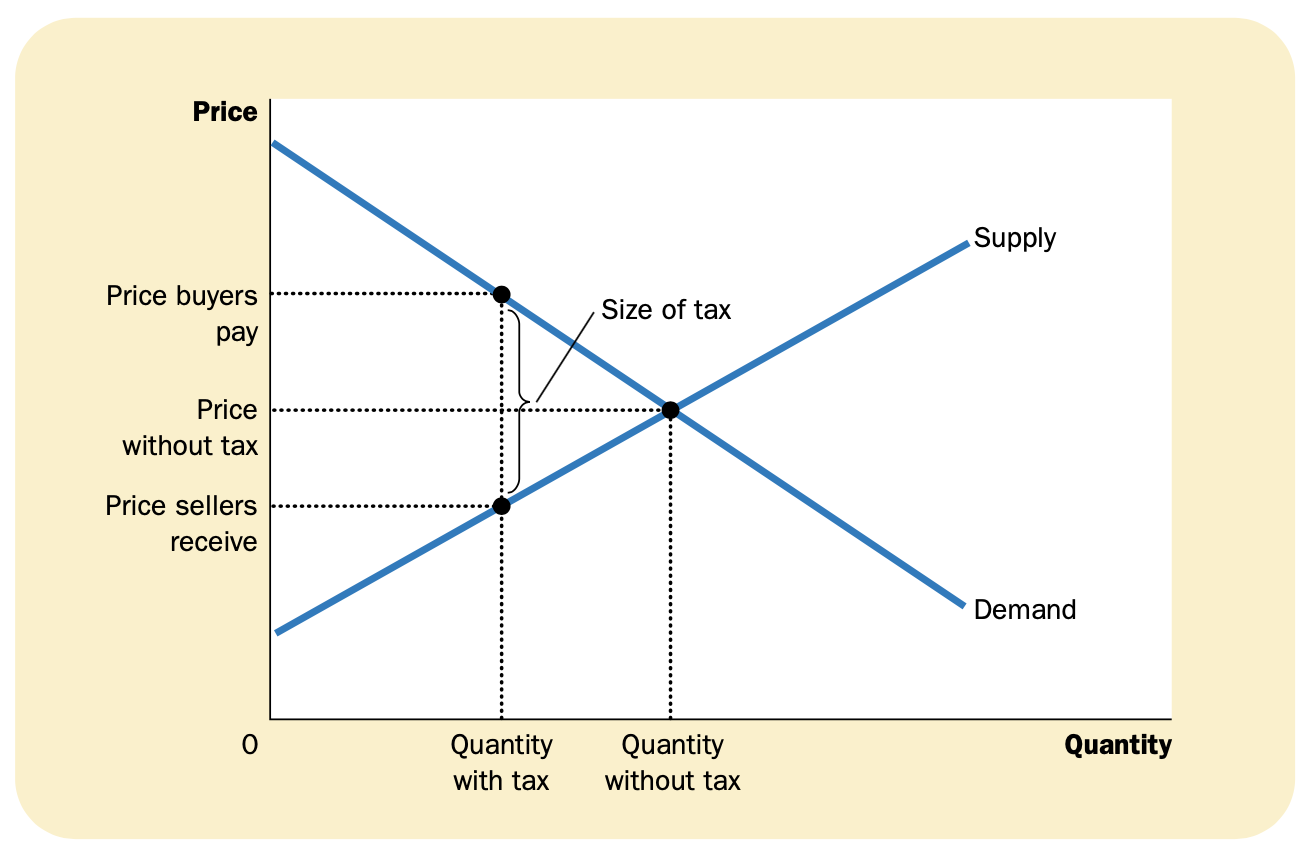
\includegraphics[width=\textwidth]{pics/the-effect-of-a-tax}
  \caption{The effect of a tax}
  \label{fig:the-effect-of-a-tax}
\end{figure}


\subsection{How a tax affects market participants}

Figure \ref{fig:tax-revenue} show the tax renenue.

\begin{figure}[!ht]
  \centering
  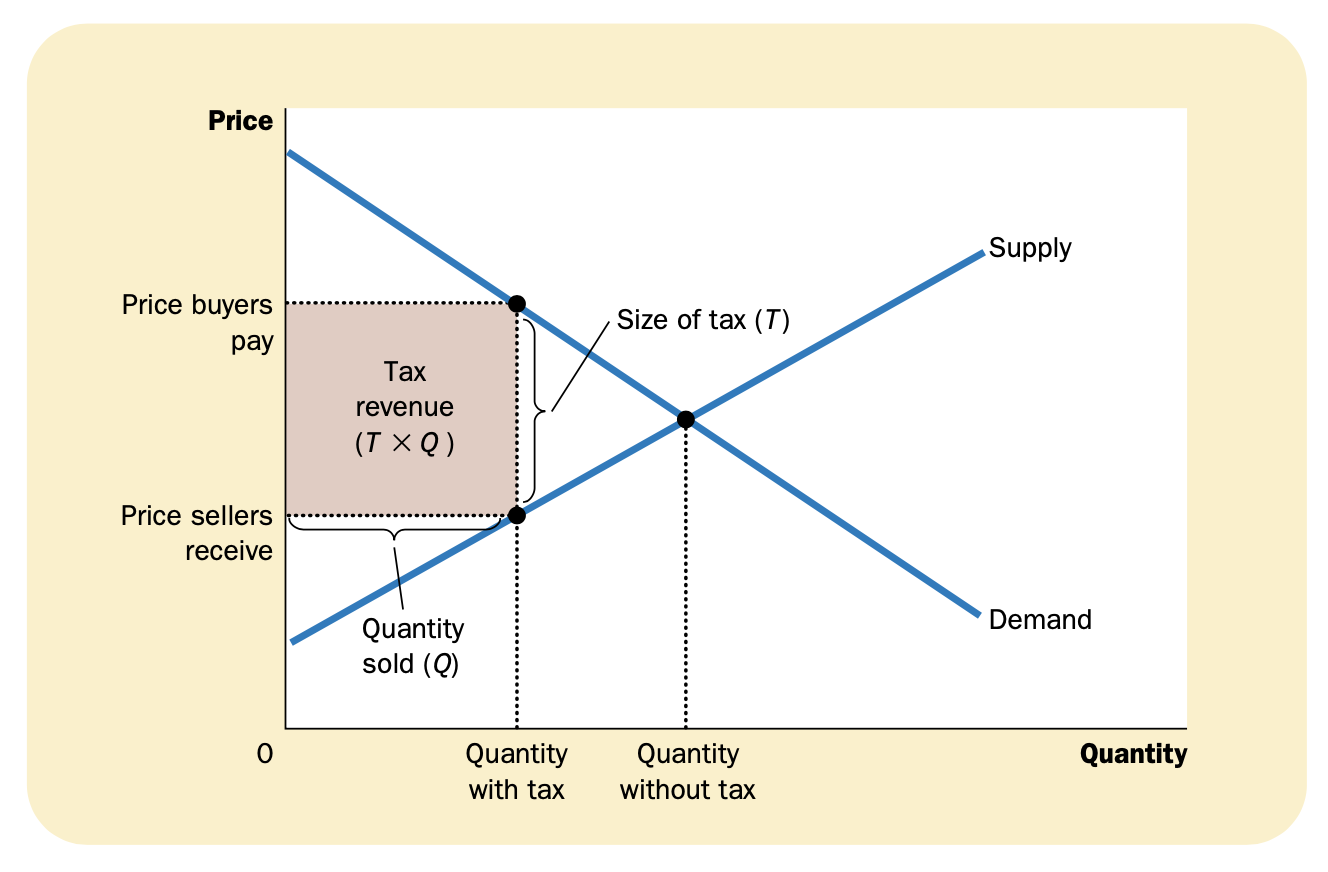
\includegraphics[width=\textwidth]{pics/tax-revenue}
  \caption{Tax renenue}
  \label{fig:tax-revenue}
\end{figure}





\subsubsection{Welfare without a tax}

Figure \ref{fig:how-a-tax-affects-welfare} shows the supply-and-demand diagram and marks the key areas with the letters A through F.

\begin{figure}[!ht]
  \centering
  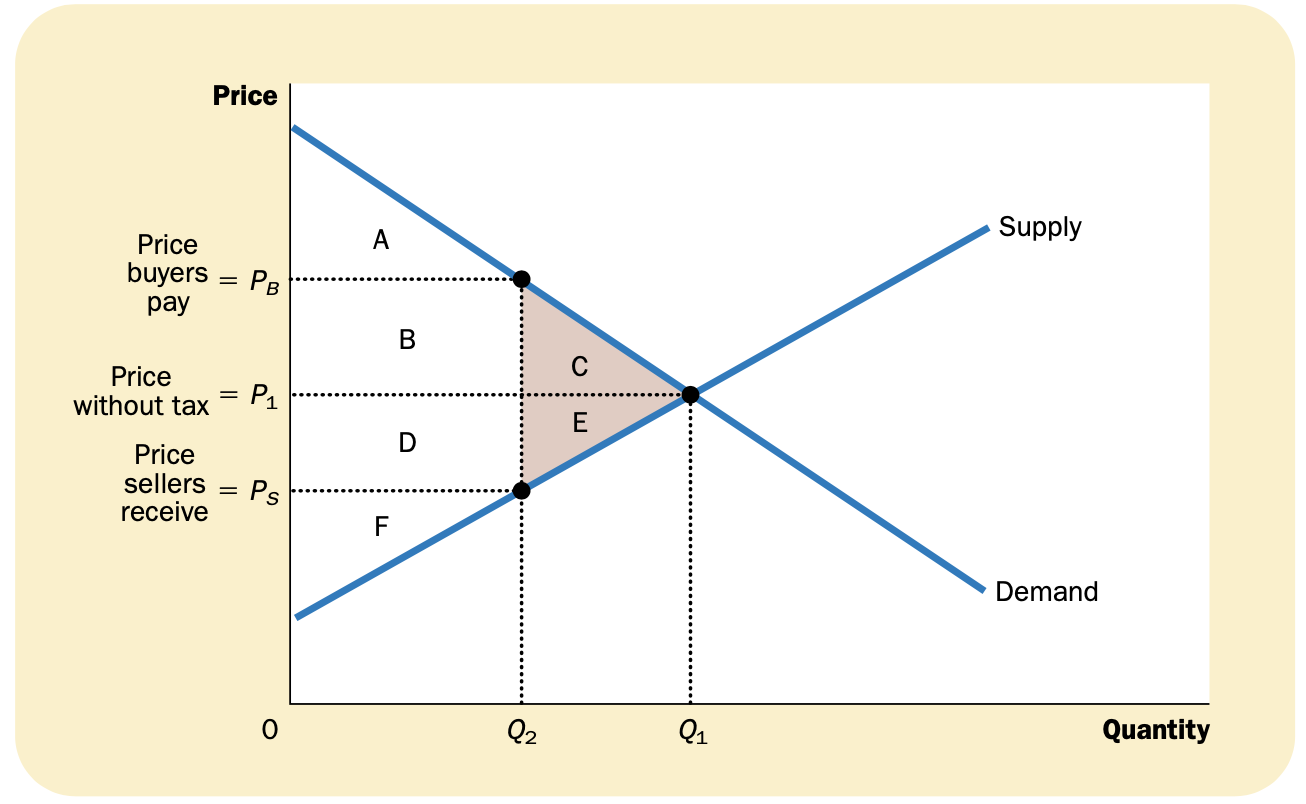
\includegraphics[width=\textwidth]{pics/how-a-tax-affects-welfare}
  \caption{How a tax affects welfare}
  \label{fig:how-a-tax-affects-welfare}
\end{figure}


Without a tax, the total surplus is : A + B + C + D + E + F.

\subsubsection{Welfare with a tax}

To compute total surplus with the tax, we add consumer surplus, producer surplus, and tax revenue.
Thus, we find that total surplus is area A + B + D + F.


\subsubsection{Change in welfare}

Total surplus in the market falls by the area C + E.
Thus, the losses to buyers and sellers from a tax exceed the revenue raised by the government.
The fall in total surplus that results when a tax (or some other policy) distorts a market outcome is called the \keyword{deadweight} loss.
The area C + E measures the size of the deadweight loss.


To understand why taxes impose deadweight losses, recall one of the Ten Principles of Economics: People respond to incentives.
Markets normally allocate scarce resources efficiently.
That is, the equilibrium of supply and demand maximizes the total surplus of buyers and sellers in a market.
When a tax raises the price to buyers and lowers the price to sellers, however, it gives buyers an incentive to consume less and sellers an incentive to produce less than they otherwise would.
As buyers and sellers respond to these incentives, the size of the market shrinks below its optimum.
Thus, because taxes distort incentives, they cause markets to allocate resources inefficiently.



\subsection{Deadweight losses and the gains from trade}


To gain some intuition for why taxes result in deadweight losses, consider an example.
Imagine that Joe cleans Jane’s house each week for \$100.
The opportunity cost of Joe’s time is \$80, and the value of a clean house to Jane is \$120.
Thus, Joe and Jane each receive a \$20 benefit from their deal.
The total surplus of \$40 measures the gains from trade in this particular transaction.

Now suppose that the government levies a \$50 tax on the providers of cleaning services.
There is now no price that Jane can pay Joe that will leave both of them better off after paying the tax.
The most Jane would be willing to pay is \$120, but then Joe would be left with only \$70 after paying the tax, which is less than his \$80 opportunity cost.
Conversely, for Joe to receive his opportunity cost of \$80, Jane would need to pay \$130, which is above the \$120 value she places on a clean house.
As a result, Jane and Joe cancel their arrangement. Joe goes without the income, and Jane lives in a dirtier house.


Figure \ref{fig:the-deadweight-loss} show the deadweight loss.

\begin{figure}[!ht]
  \centering
  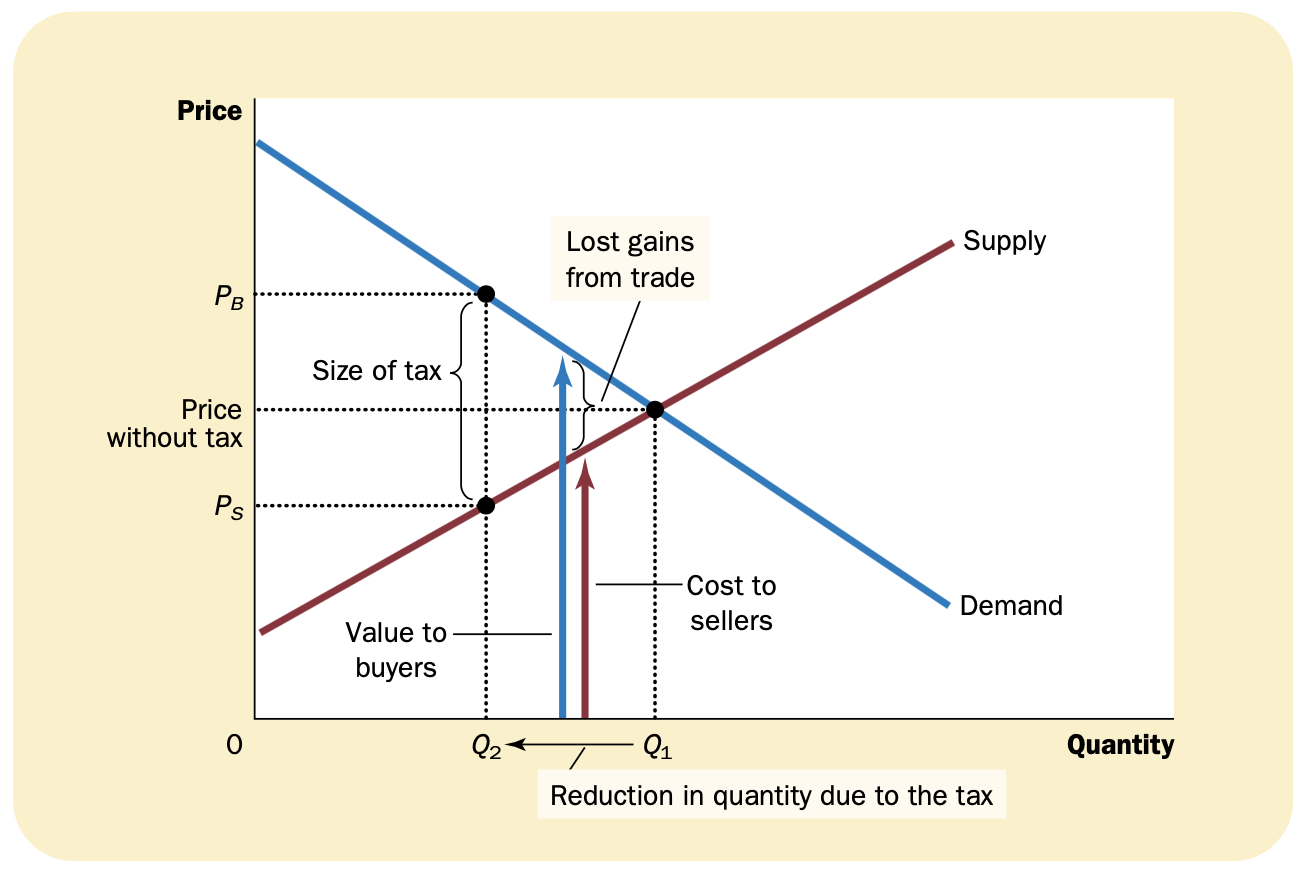
\includegraphics[width=\textwidth]{pics/the-deadweight-loss}
  \caption{The deadweight loss}
  \label{fig:the-deadweight-loss}
\end{figure}


From this example, we can see the ultimate source of deadweight losses: Taxes cause deadweight losses because they prevent buyers and sellers from realizing some of the gains from trade.



\section{The determinants of the deadweight loss}

What determines whether the deadweight loss from a tax is large or small?

The answer is the price elasticities of supply and demand, which measure how much the quantity supplied and quantity demanded respond to changes in the price.
This is shown in Figure \ref{fig:tax-distortions-and-elasticities}.
\begin{figure}[!ht]
  \centering
  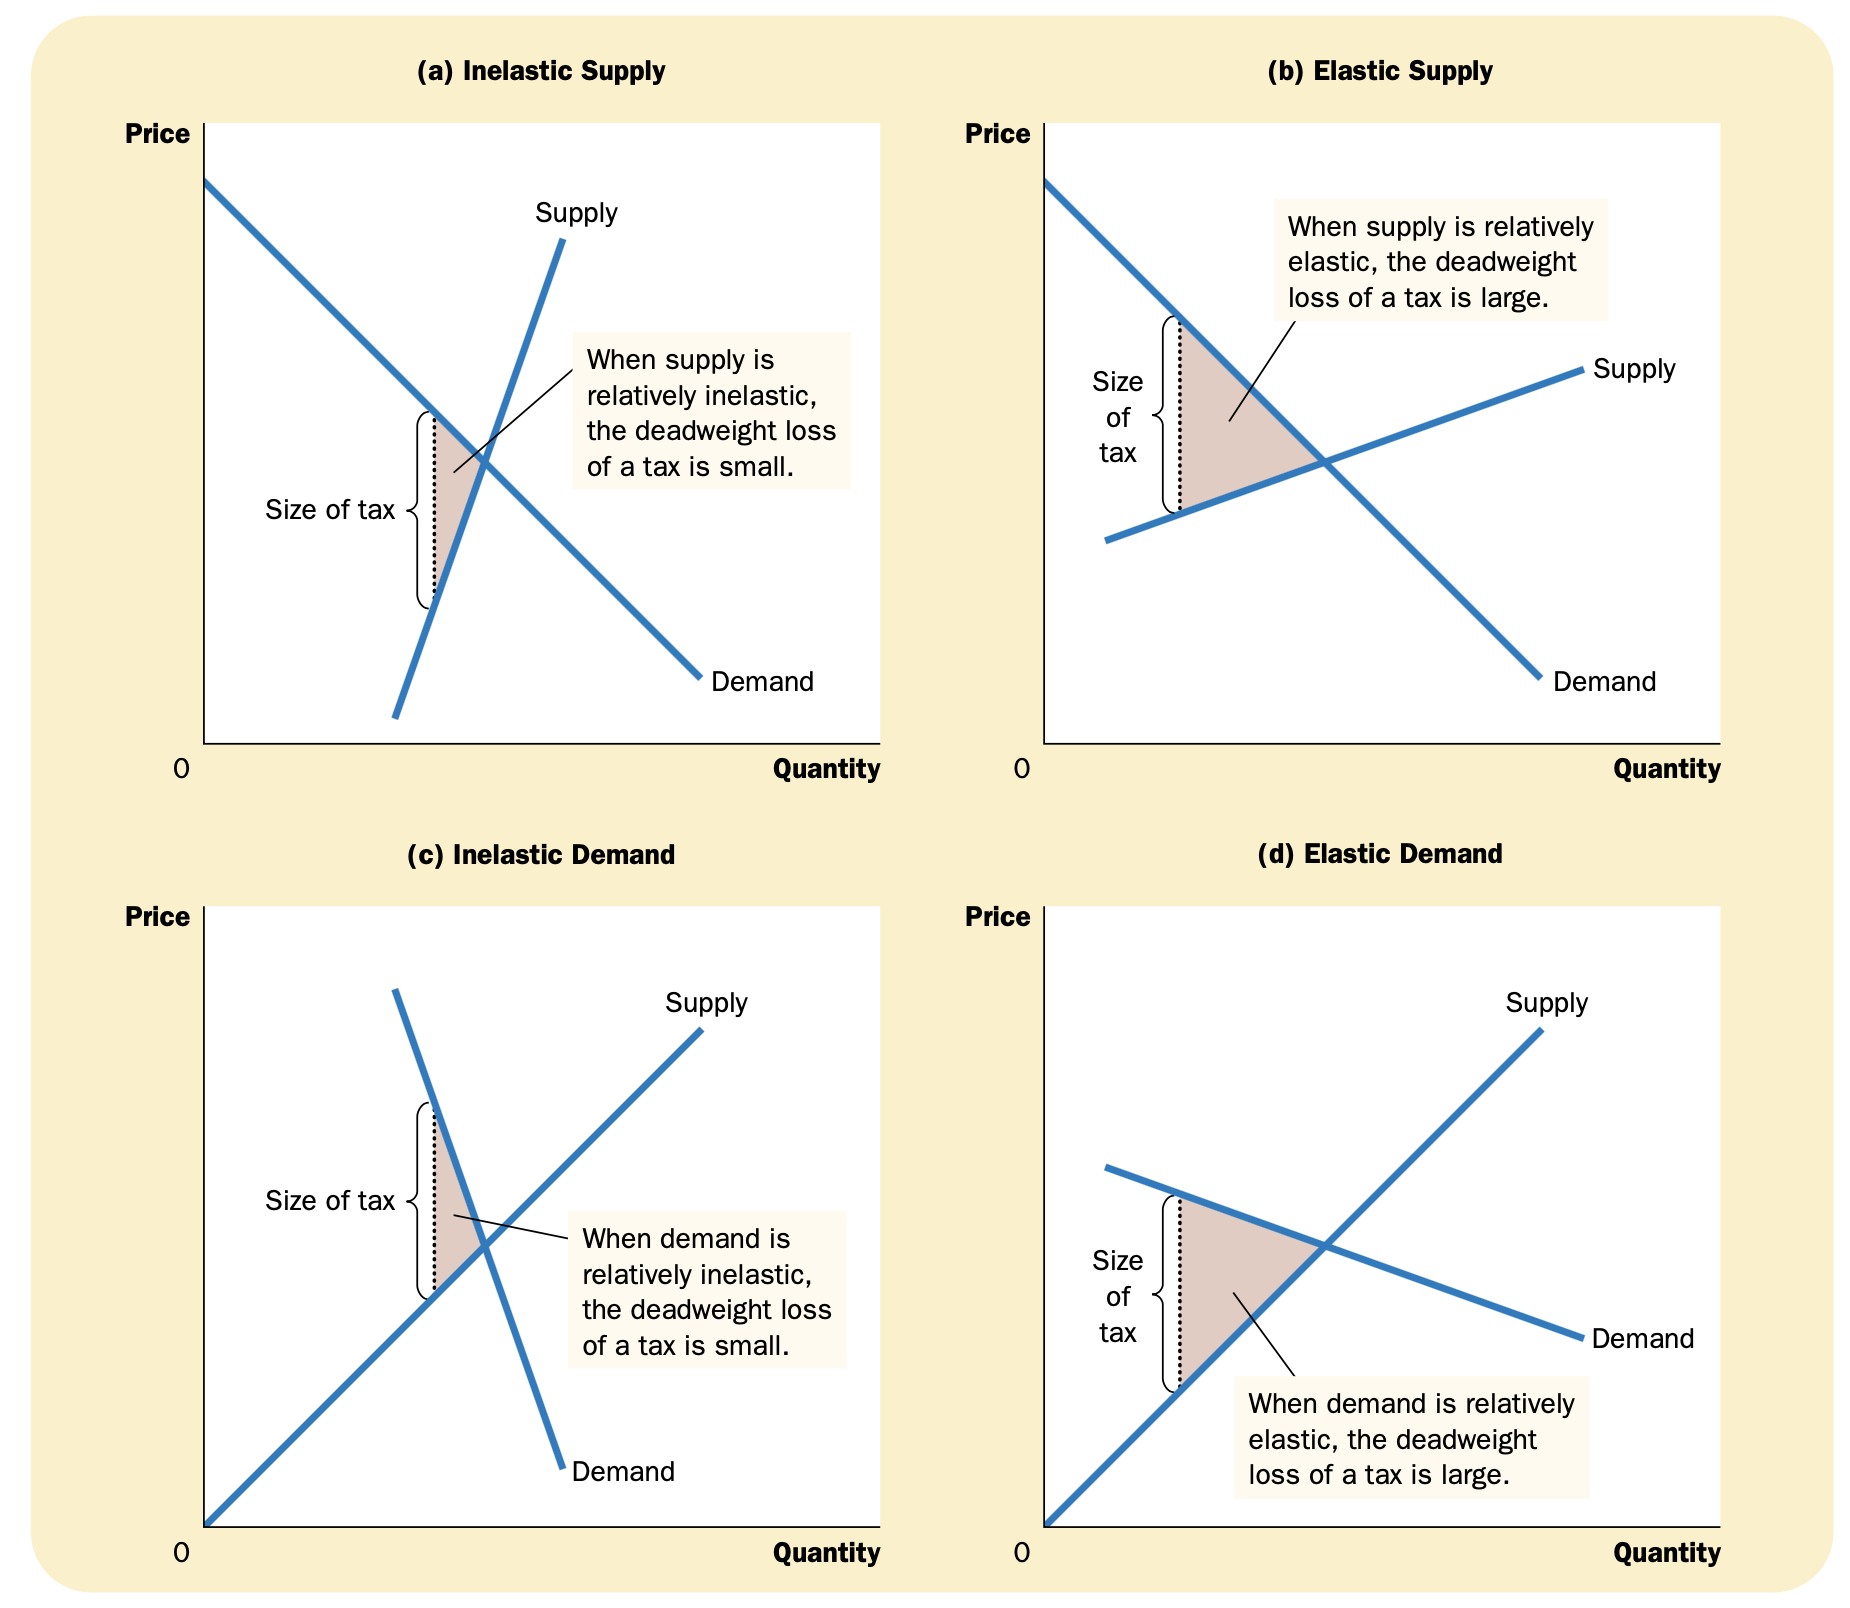
\includegraphics[width=\textwidth]{pics/tax-distortions-and-elasticities}
  \caption{Tax distortions and elasticities}
  \label{fig:tax-distortions-and-elasticities}
\end{figure}


\section{Deadweight loss and tax revenue as taxes vary}

Figure \ref{fig:taxes-vary} shows the effects of a small, medium, and large tax, holding con- stant the market’s supply and demand curves. 

\begin{figure}[!ht]
  \centering
  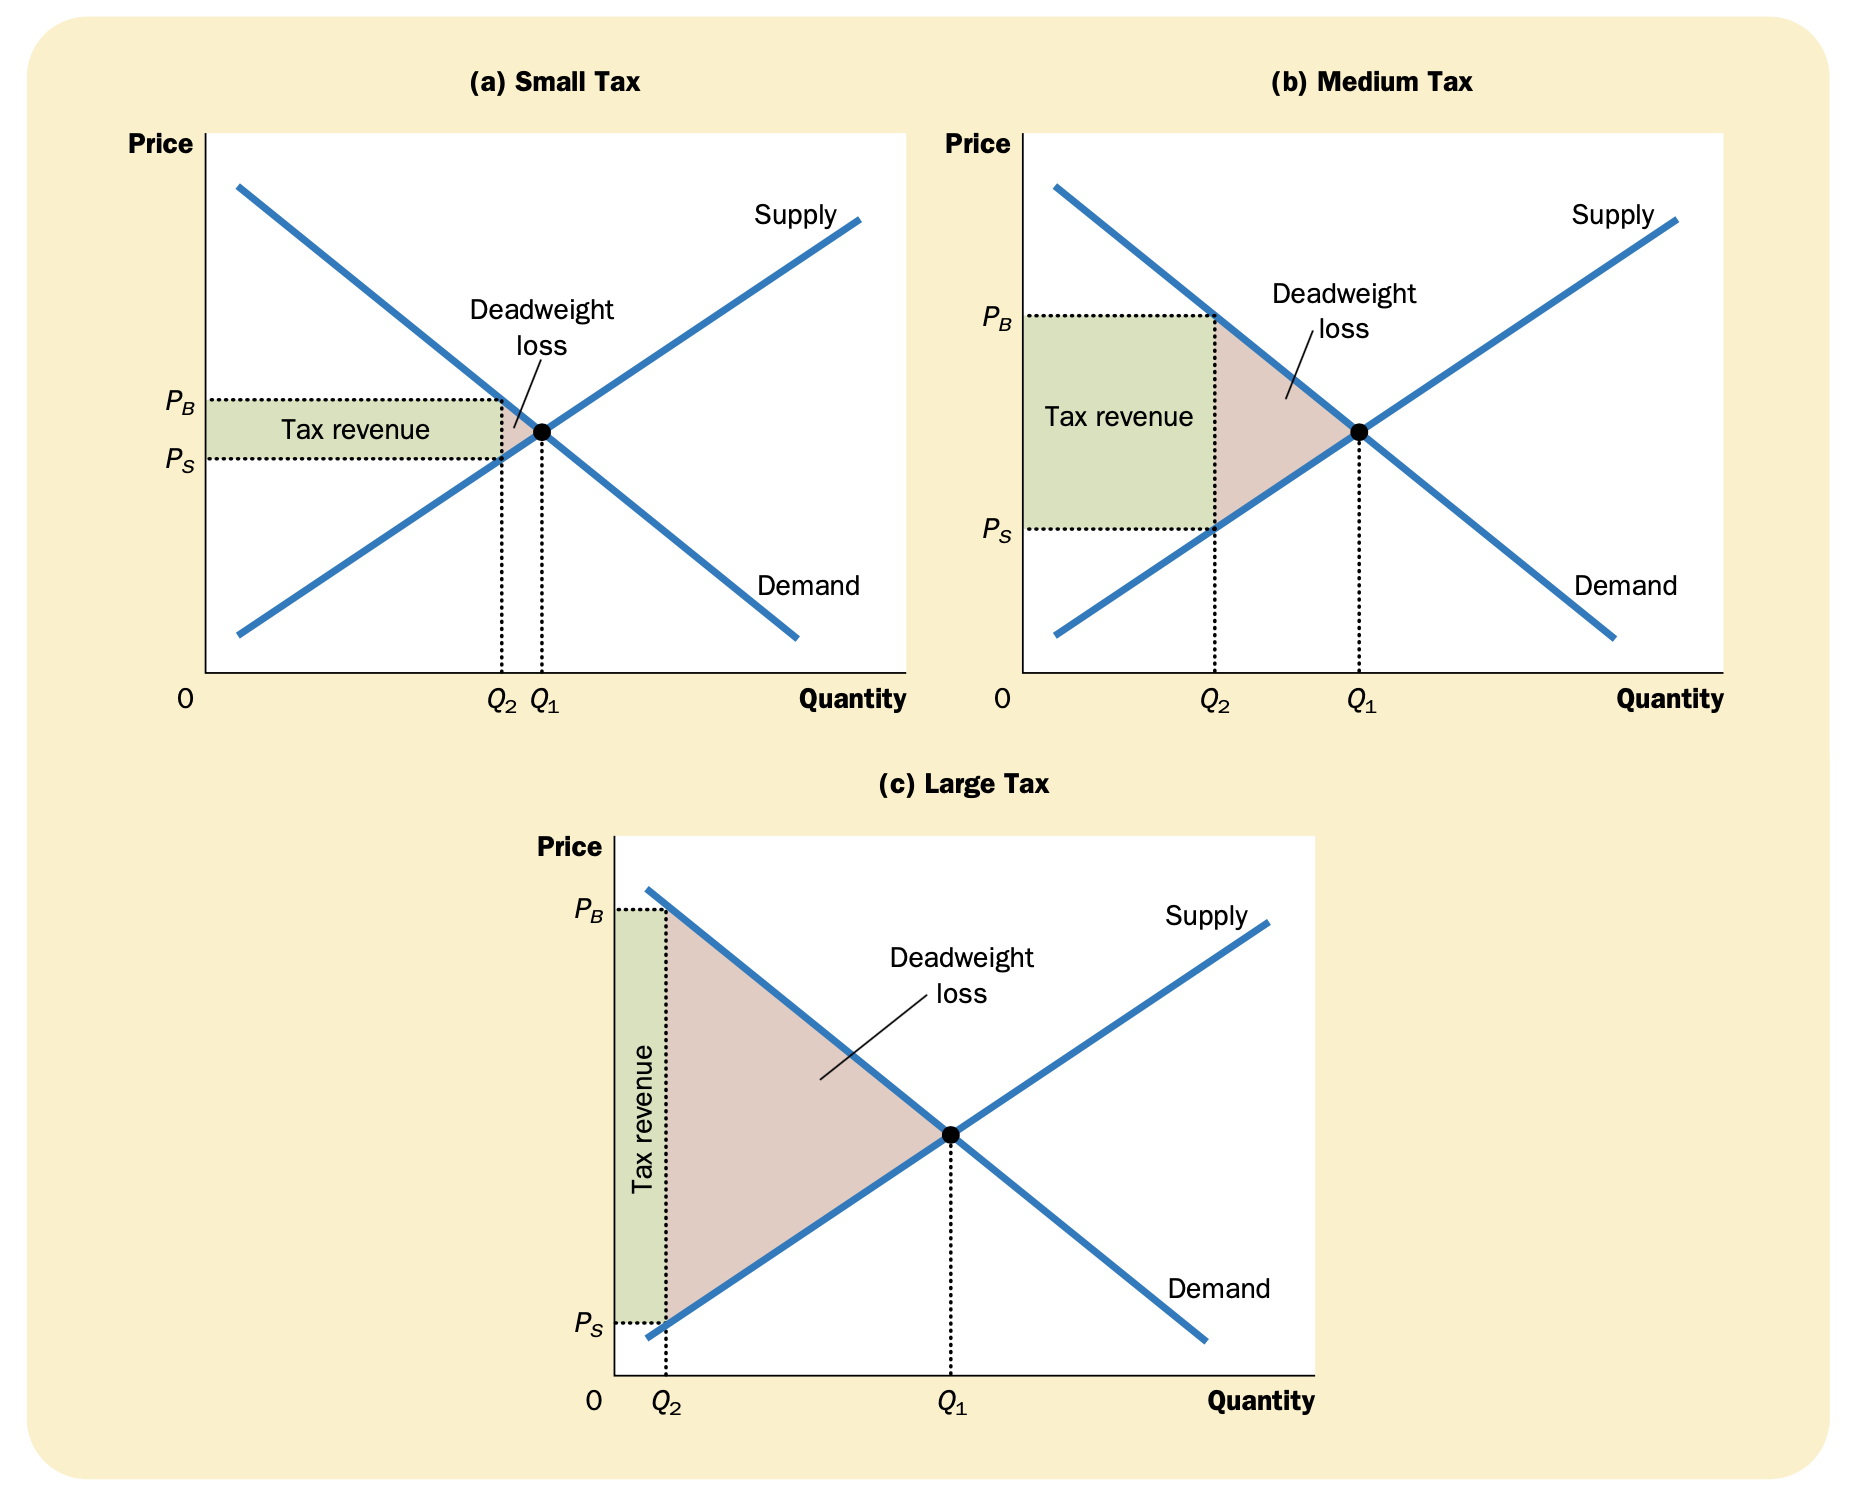
\includegraphics[width=\textwidth]{pics/taxes-vary}
  \caption[Taxes vary]{Deadweight loss and tax revenue as taxes vary}
  \label{fig:taxes-vary}
\end{figure}

Figure \ref{} summarizes these results.
In panel (a) we see that as the size of a tax increases, its deadweight loss quickly gets larger.
By contrast, panel (b) shows that tax revenue first rises with the size of the tax; but then, as the tax gets larger, the market shrinks so much that tax revenue starts to fall.

\begin{figure}[!ht]
  \centering
  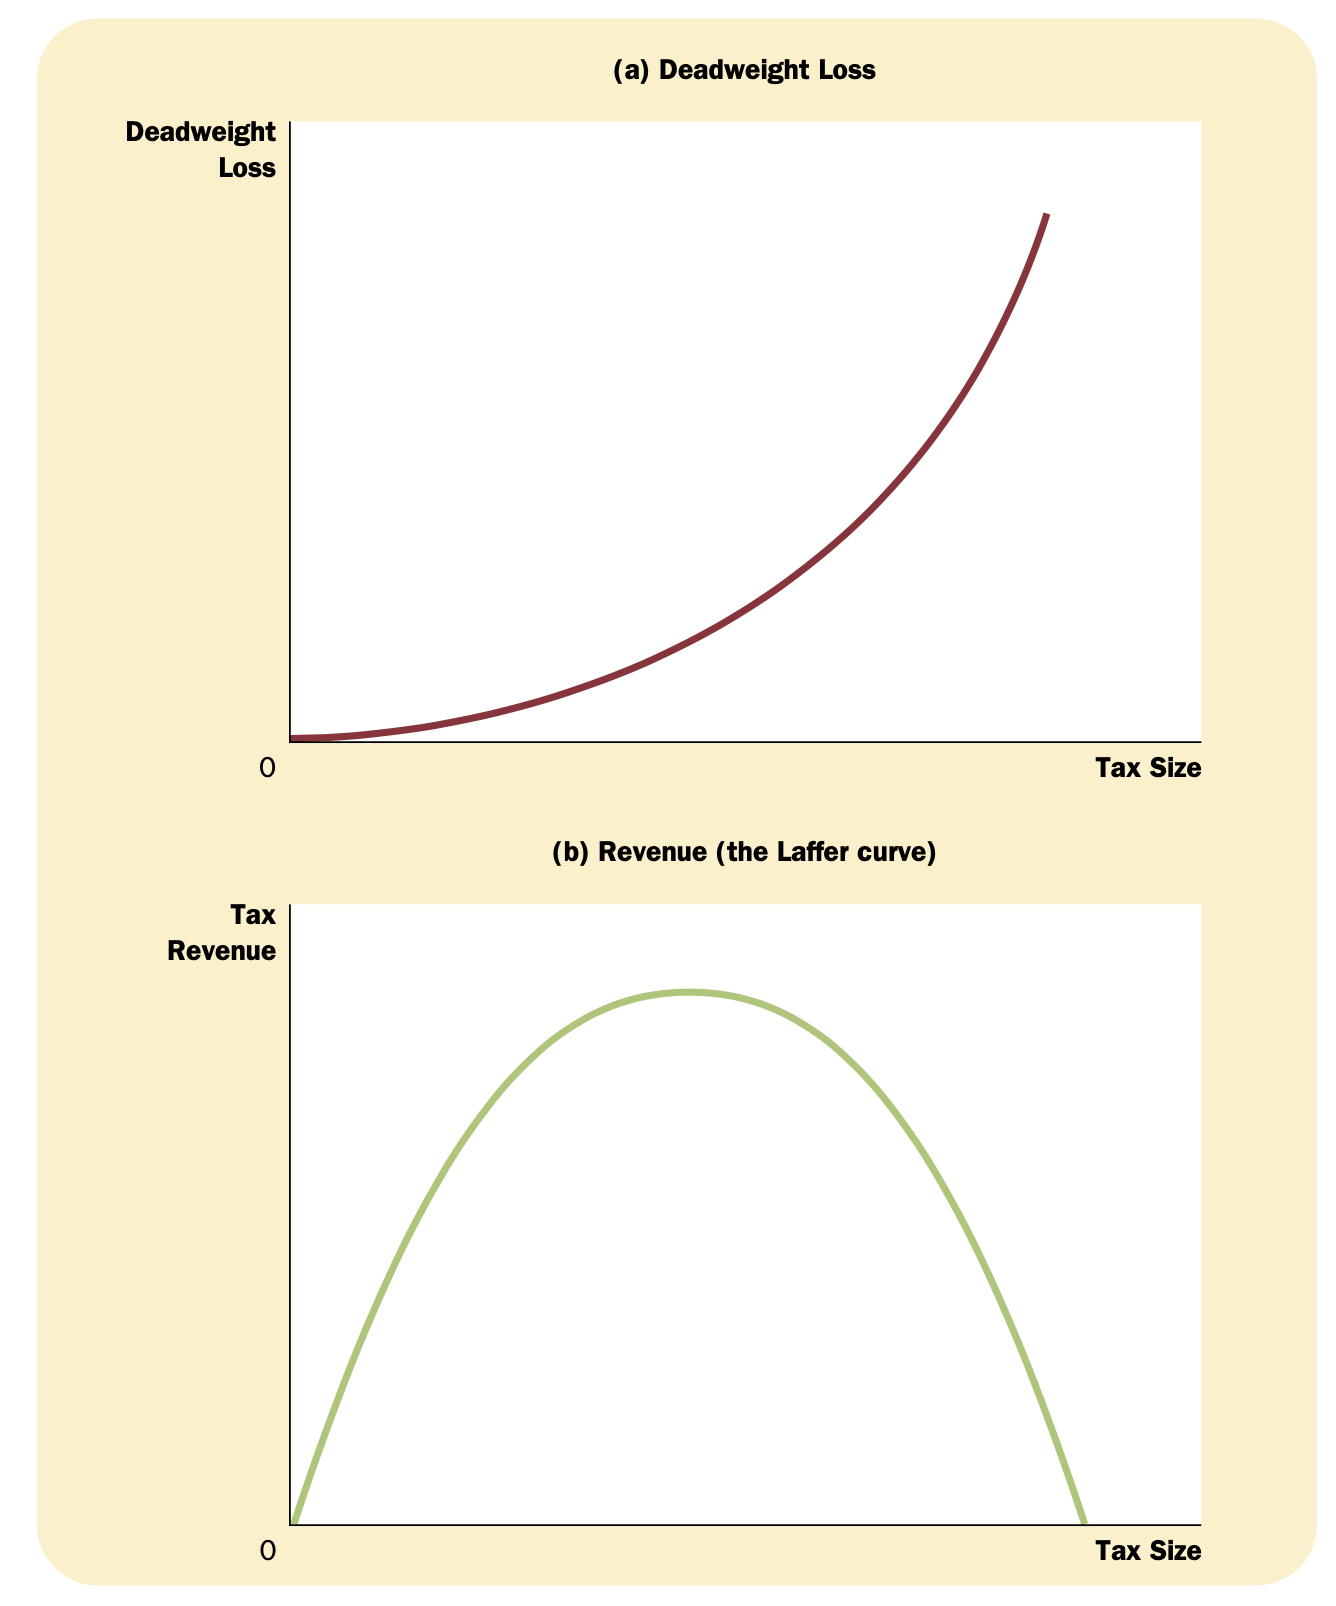
\includegraphics[width=\textwidth]{pics/deadweight-loss-and-tax-revenue-vary}
  \caption[Size of tax]{How deadweight loss and tax revenue vary with the size of a tax}
  \label{fig:size-of-tax}
\end{figure}



\section{Conclution}

Taxes, Oliver Wendell Holmes once said, are the price we pay for a civilized society.
Indeed, our society cannot exist without some form of taxes.
We all expect the government to provide certain services, such as roads, parks, police, and national defense.
These public services require tax revenue.



Markets are usually a good way to organize economic activity.
When the government imposes taxes on buyers or sellers of a good, however, society loses some of the benefits of market efficiency.
Taxes are costly to market participants not only because taxes transfer resources from those participants to the government, but also because they alter incentives and distort market outcomes.